\chapter{Introduction}\label{ch:introduction}
\section{Context and motivation}
Since the term \emph{\gls{ai}} was coined at the Dartmouth Conference in 1956~\cite{mccarthy2006proposal} until nowadays, this field of computer science has developed at a great pace. During this time, its contributions to robotics and computer vision have brought machines that can solve certain tasks as well as humans and, in some cases, even surpass human performance. In order to understand the context in which this project has been developed, the fields and subfields that have led to the birth of \emph{\glspl{cnn}} are going to be defined, trying to clarify the differences between them and how they are related to each other. 
\begin{description}
	\item[Artificial intelligence.] ``It is the subfield of computer science devoted to developing programs that enable computers to display behavior that can (broadly) be characterized as \emph{intelligent}"~\cite{sep-logic-ai}. In this definition, intelligent refers to the ability of perceiving the environment and acting consequently, trying to maximize the chances of achieving a certain goal~\cite{Russell:2003:AIM:773294}.
\end{description}
\begin{description}
	\item[Machine learning.] According to a quote attributed to Arthur Samuel, it is the ``field of study that gives computers the \emph{ability to learn} without being \emph{explicitly programmed}"\cite{ml-def}. Given this definition, it can be asserted that \gls{ml} is a subfield of \gls{ai}, because computers that have the ability to learn will exhibit an intelligent behaviour, but displaying an intelligent behaviour doesn't necessarily mean to learn. For instance, \emph{Deep Blue} chess-playing system can be considered intelligent as it achieves a \emph{human comparable performance}, but instead of actually learning to play, it was hard-coded with a function that evaluated the board positions~\cite{Goodfellow-et-al-2016}. Machine learning algorithms can be divided in two main groups:
	\begin{itemize}
		\item \textbf{Supervised learning}. Given a training set of N example input–output pairs $(x_1, y_1),(x_2, y_2), . . .(x_N, y_N)$, where each $y_j$ was generated by an unknown function $y = f(x)$, supervised learning algorithms try to find a function $h$ that approximates the true function $f$\cite{Russell:2003:AIM:773294}. The example inputs and their outputs are usually called samples and labels, respectively.
		\item \textbf{Unsupervised learning}. In this case, example inputs $x_j$ are provided without their corresponding outputs $y_j$. The goal of these algorithms is to find a function that describes some underlying structure in data\cite{unsup}. 
	\end{itemize}
	The main challenge of \gls{ml} is \emph{generalization}, that is, ``the ability to perform well on previously unobserved inputs"\cite{Goodfellow-et-al-2016}. By contrast, if the algorithm learns to generate correct outputs for already seen inputs, but not for unseen ones, it is said to \emph{overfit}. In \gls{ml}, the example inputs are usually \emph{vectors of features} extracted from data. These example inputs, and their corresponding outputs in the case of supervised learning, are treated as \emph{training data}. As the training process is \emph{iterative}, some examples are usually kept as \emph{validation data}, which is used to evaluate the algorithm performance during training. Validation is usually employed to stop training when a certain criteria is met, avoiding overfitting. When the training process finishes, \emph{test data}, formed by unseen samples, is fed to the algorithm to evaluate its performance.
\end{description}
\begin{description}
	\item[Artificial neural networks.] They are a computational approach that tries to model the way a \emph{biological neural network} solves problems\cite{Goodfellow-et-al-2016}. As it can be seen in Figure~\ref{fig:ANN}, they're formed by layers of interconnected \emph{neural units}.
	\begin{figure}
		\centering
		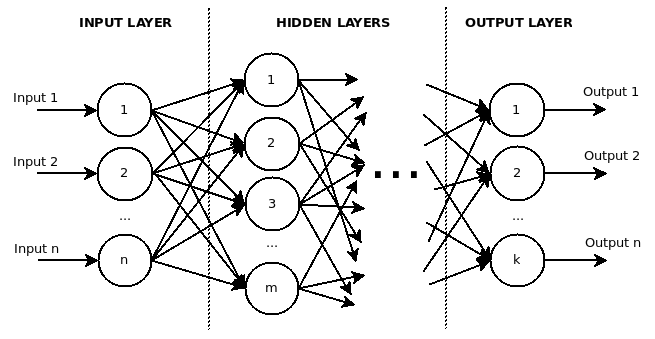
\includegraphics[width=0.8\linewidth, keepaspectratio]{figures/ANN.png}
		\caption{Basic architecture of an artificial neural network.}
		\label{fig:ANN}
	\end{figure}
	
	In \glspl{ann}, each neural unit sums the weighted input signals and apply an \emph{activation function} that can be linear or non-linear (see Figure~\ref{fig:unit}). The result of this operation is transferred to the neurons of the next layer. During training, weights are updated based on a \emph{learning rule} that will try to minimize the difference between the current output and the desired one. As \glspl{ann} are able to learn from experience, they're classified within the \gls{ml} field. It is important to clarify that if an \gls{ann} employs only linear activation functions, it will only be able to solve linearly separable problems. The usage of non-linear activation functions allows the settlement of more complex tasks. Examples for both cases are shown in Figure\ref{fig:linear}.	
	\begin{figure}
		\centering
		\includegraphics[width=0.8\linewidth, keepaspectratio]{figures/unit.png}
		\caption{A neural unit (source~\cite{neural-unit}).}
		\label{fig:unit}
	\end{figure}
	\begin{figure}
		\centering
		\includegraphics[width=0.9\linewidth, keepaspectratio]{figures/linear.png}
		\caption{Example of linearly and non-linearly separable problems.}
		\label{fig:linear}
	\end{figure}
\end{description}
\begin{description}
	\item[Deep learning.] It is a branch of \gls{ml} which is based on algorithms that share the following properties~\cite{deep-learning-methods-and-applications}:
	\begin{itemize}
		\item \emph{Multiple layers} of \emph{non-linear} processing units.
		\item The supervised or unsupervised \emph{hierarchical learning} of feature representations in each layer.
	\end{itemize}
	
	Although the term \textit{deep learning} is not explicitly linked to \glspl{ann}, in practice we could talk about deep learning as a subset of neural networks algorithms that share the properties mentioned above. With deep learning algorithms, it is no longer necessary to extract a vector of features to represent the input data, as these algorithms have the ability of learning, not only how to generate a correct output, but also how to represent data in a hierarchical way.
\end{description}
\begin{description}
	\item[Convolutional neural networks.] They are ``neural networks that use \emph{convolution} in place of general matrix multiplication in at least one of their layers"~\cite{Goodfellow-et-al-2016}. \glspl{cnn} are deep learning algorithms which are specifically designed to process data that has a \emph{grid-like topology}, like images and audio. In a few years, they have become one of the most promising subfields of \gls{ml}, outperforming the results achieved by the previous algorithms in the most popular benchmarks for tasks like object classification, object detection and natural language processing. The details about how \glspl{cnn} work will be the deeply discussed in the following chapters.
\end{description}

\begin{description}
	\item[Computer vision.] It is a field of computer science which ``aims to build \emph{autonomous systems} which could perform some of the tasks that the \emph{human visual system} can perform"~\cite{huang1996computer}. In order to build autonomous systems, computer vision applications have to deal with image acquisition, processing and analysis. Computer vision has always been closely related to \gls{ai} and \gls{ml}, and in the last years, the integration of deep learning algorithms (e.g. \glspl{cnn}) in computer vision applications has led to major advances in the field.
\end{description}

There are multiple \emph{motivations} behind this project. On the one hand, I am very passionate about \emph{computer vision}, because of its great implications in everyday life. For instance, it is involved in medical imaging, surveillance, augmented reality, automatic inspection in manufacturing, self-driving cars... and the list goes on and on. On the other hand, applications that have just been mentioned, have benefited from the inclusion of \emph{deep learning} in computer vision. It is really exciting to see how many researchers are currently working in the field. Of course, this is not a coincidence. The great results achieved with these new algorithms has boosted the growth of \gls{ai} in the last years and has normalized its usage in \emph{commercial applications}. However, everything has its ups and downs. There are lots of people worried about the so-called \emph{\textit{black box} problem} in deep learning~\cite{black-box}, i.e., how machines are actually learning to do what they do. In this work, besides developing a real-world application to show how powerful \glspl{cnn} are, we're going to try to cast some light into the aforementioned \textit{black box}. 

\section{Objectives}\label{sec:objectives}
The ultimate objective of this project is to fully understand \glspl{cnn} in order to integrate them in a computer vision application that must be able to solve a real-world task, specifically a \emph{real-time handwritten digits classifier}. This main objective has been divided in the following sub-objectives: 
\begin{itemize}
	\item Accomplishing a \emph{deep understanding} of how a basic \gls{cnn} works, analyzing its main layers, the learning process and the particularities of building this kind of networks with \emph{Keras}, a neural network library for Python.
	\item Building a \emph{component} which integrates a \gls{cnn} to classify images of handwritten digits in real time.
	\item Developing a \emph{test bench} which allows the comparison of the performance achieved by the \glspl{cnn}. This test bench must provide the input data and the tools required to visualize and evaluate the results.
	\item Studying the \emph{effects of the learning process} in the performance of \glspl{cnn} trained with different datasets, architectures and regularization methods.
\end{itemize}

\section{Methodology}
The development of this project has been weekly followed by the tutors. In the \emph{weekly meetings} the work done in the previous week was discussed and new milestones were set for the following one. This methodology has allowed a continuous feedback, which has led to a better understanding of the topic. Besides that, thanks to the weekly meetings the workload has been constant during these months. 

Additionally, the following tools have been employed to keep track of the project progress:
\begin{itemize}
	\item \textbf{GitHub}. All the code written in this project is available in GitHub and has been  frequently updated. In the following link, the main repository can be accessed:
	\url{https://github.com/RoboticsURJC-students/2016-tfg-david-pascual}
	\item \textbf{MediaWiki}. It has been used as a logbook of the progress of this project. It can be accessed in the following link:
	\url{http://jderobot.org/Dpascual-tfg}
\end{itemize}

In Figure~\ref{fig:gantt}, a \emph{Gantt chart} with the number of weeks dedicated to every task in the project can be seen.
\begin{figure}
	\centering
	\includegraphics[width=0.9\linewidth, keepaspectratio]{figures/gantt.png}
	\caption{Gantt chart.}
	\label{fig:gantt}
\end{figure}

\section{Project structure}
For ease of reading, the structure followed in the writing of this document and how the chapters are related to each other are explained in this section.

\begin{description}
	\item[Chapter 1. Introduction.] This chapter starts with a brief introduction to the main fields in which \glspl{cnn} are based and the motivations behind the project. Then, the objectives, the methodology followed to meet these objectives and the structure of the project are presented.
	\item[Chapter 2. Framework.] The third-party software that has supported the development of this project is described here. It's specially significant the section about Keras library, its main functionalities and the theory behind its core layers and learning process.
	\item[Chapter 3. Digit classifier.] In this chapter, an example of a \gls{cnn} built with Keras for handwritten digits classification is analyzed. Then, the internals of the developed component, in which the \gls{cnn} is integrated, are explained.
	\item[Chapter 4. Test bench.] The datasets that will be used for training new models and the tools that will be employed to evaluate and visualize the results are described in this chapter.
	\item[Chapter 5. Evaluation.] Taking as a starting point the \gls{cnn} that was analyzed in the \textit{Digit classifier} chapter, new models will be created. The performance of these new models will be evaluated with the tools developed in the \textit{Test bench} chapter.
	\item[Chapter 6. Conclusions.] Finally, the conclusions reached during the development of this project will be summarized and possible further works will be proposed.
\end{description}
